\section{The Radiation Belts}
The term ``Radiation Belts'' or ``Van Allen belts'' refer to the trapped distributions of sparse, very-high-energy electrons, which exhibit two shell-like enhancements which comprise the inner and outer radiation belts. First measured in 1958 by Geiger counters aboard satellites 1958$\alpha$ and 1958$\gamma$ of the Explorer program, the radiation belts were one of the earliest discoveries of the American space program \citep{VanAllen1958}. The vast majority of plasmasphere electrons are ``cold'', and have kinetic energies well under $\sim$ 1 eV. However, radiation belt electrons, while sparse in density, can be highly relativistic, with energies approaching 10 MeV.

Section \ref{section:plasmasphere_density_models} describes the density of electrons and ions in the near-Earth environment. Absent from these models, however, is a discussion of electron and ion energies. The model in section \ref{section:thermal_electron_distributions} assigns an energy distribution to electrons in the $\sim$ 1 eV range to model a warm plasma; the higher energies of radiation belt electrons, however, necessitate a different model.

We model the trapped electron population using the AE8 density model \citep{Vette1991}. AE8 provides omnidirectional, integral fluxes of high-energy electrons as a function of L-shell energy. AE8 is the culmination of several decades of radiation belt studies by the National Space Science Data Center (NSSDC), with the first efforts originating with \cite{Vette1966}. AE8 combines measurements from $\sim$ 94 different instruments across $\sim$ 24 satellite missions from the 1960s and 1970s, which spanned a wide range of orbits, from LEO out to geostationary \citep{Cayton2005}.

Figure \ref{fig:AE8_model} shows the AE8 model output for minimally-populated and maximally-populated conditions. 

\begin{figure}
\begin{center}
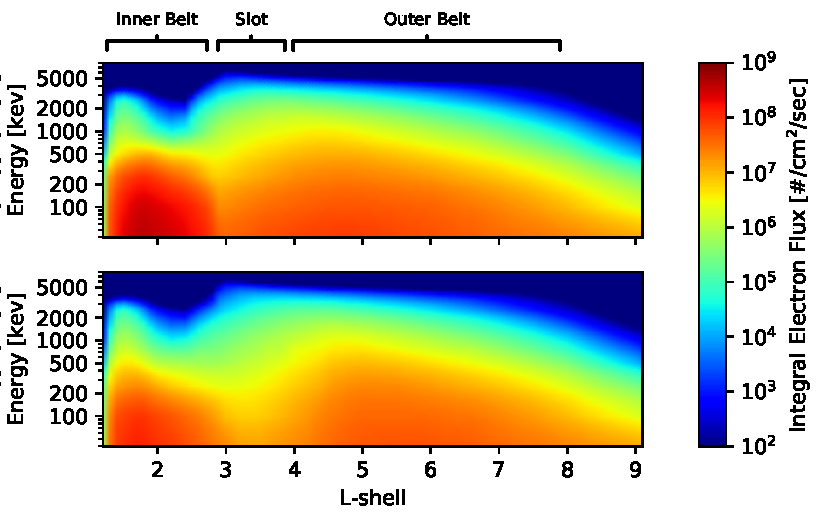
\includegraphics{figures/AE8_fluxes.pdf}
\caption[AE8 integral flux model]{Integral flux for energetic electrons in the radiation belts, as reported by the AE8 model \citep{Vette1991}. The top frame shows the model of maximum conditions, and the bottom frame minimum conditions. The two radiation belts are visible as enhancements within L$\approx$ 2 -- 3 for the inner belt, and L$\approx$ 4 -- 7 for the outer belt. The belts are separated by a depletion known as the ``slot'' region.}
\label{fig:AE8_model}
\end{center}
\end{figure}

The AE8 model reports omnidirectional, integral fluxes -- that is, the total electron flux integrated over a spherical surface -- at the geomagnetic equator. However we require finer detail in directional flux of electrons, which we model via a distribution of pitch angles. \cite{Lauben1998} assumed the simplest distribution, with electrons uniformly-distributed in pitch angle up to the loss cone. \cite{Bortnik2005} compared the square distribution to a more-realistic, sinusoidal distribution. Here we assume a sinusoidal pitch-angle distribution along with the AE8 flux density model. Figure \ref{fig:pitchangledistributions} contrasts the square and sinusoidal distribution functions.


\begin{figure}
\begin{center}
\includegraphics{figures/pitch-angle_distributions.pdf}
\caption[Pitch-angle distribution functions]{Two models of the distribution in pitch angle of radiation belt electrons. The simplest model is a square-shaped distribution, wherein pitch-angles are equally represented within the trapped population. A more realistic model is a sinusoidal distribution. Densities within the loss cone ($\alpha < \alpha_{lc}$) are assumed to be zero.}
\label{fig:pitchangledistributions}
\end{center}
\end{figure}

